\chapter{Warping der Bilder}

Sobald die Linienpaare gesetzt wurden, kann der eigentliche Algorithmus gestartet werden. Die Pixel
des Quellbildes werden in Richtung der Linienpositionen des Zielbildes verschoben. Und die Pixel
des Zielbildes wiederum werden in Richtung der Linienpositionen des Quellbildes verschoben.
Dies ist ein iterativer Prozess. Je mehr Iterationen gewählt werden, desto flie \ss ender ist
die Verzerrung.
Fuer jeden Pixel im Bild wird jede Linie in Betracht gezogen. Alle Linien haben also einen gewissen Einfluss auf
das Warping eines Pixels. Die Laufzeitkomplexitaet
des Beier-Neely Algorithmus errechnet sich aus
$\mathcal{O}(numPixels \cdot numLines)$.
Der Einfluss einer Linie auf einen Pixel kann mit einem
von Beier-Neely entwickelten Gewicht festgelegt werden
\cite{beierneely}:

\begin{equation}
	weight = \left(\frac{length^{p}}{a+dist}\right)^{b}
\end{equation}

a, b, p sind Konstanten, die einmalig gesetzt werden.

\begin{itemize}
	\item \textbf{length}: Laenge der Linie
	\item \textbf{dist}: senkrechter Abstand des Pixels zur Linie (der kürzeste Abstand
	von Punkt zu Linie).
	\item \textbf{a}: Bestimmt den Einfluss der senkrechten Distanz
	auf das Gewicht. Wenn a nahe 0 ist, so werden Pixel, die auf der
	Linie liegen mit einem Gewicht von nahezu $\infty$ beeinflusst.
	\item \textbf{b}: Kontrolliert den Fall-Off der Linien. Ist b
	nahe 0, tragen alle Linien, gleich Ihrer senkrechten Distanz zum
	Pixel, gleichmaessig zur Verzerrung des jenes Pixels bei.
	Grosse Werte (es wird nicht erwaehnt, was gross ist), fuehren
	zu einem hoeheren Gewicht, je naeher der Pixel sich an
	der jeweiligen Linie befindet.
	\item \textbf{p}: Regelt, ob sich die Linienlaenge auf das Gewicht
	auswirkt. Bei einem Wert von 0 wird $length^{p}$ offensichtlich 1
	und das Gewicht ist unabhaengig zur Linienlaenge.
\end{itemize}

Wie die Parameter festgelegt werden kommt auf die in den Bildern
vorhandenen Features an und erfordert in der Regel ein wenig
ausprobieren. Beispielsweise haben sich die Werte 
a = 0, b = 3.045 und p = 0 fuer das Bilderset aus Abbildung
\ref{fig:linepairsfinal} in unseren Tests bewaehrt.
Die Linien koennen linear interpoliert werden, wie Abbildung \ref{fig:linearinterpolation}zeigt. 
\begin{figure}[htb]
	\centering
	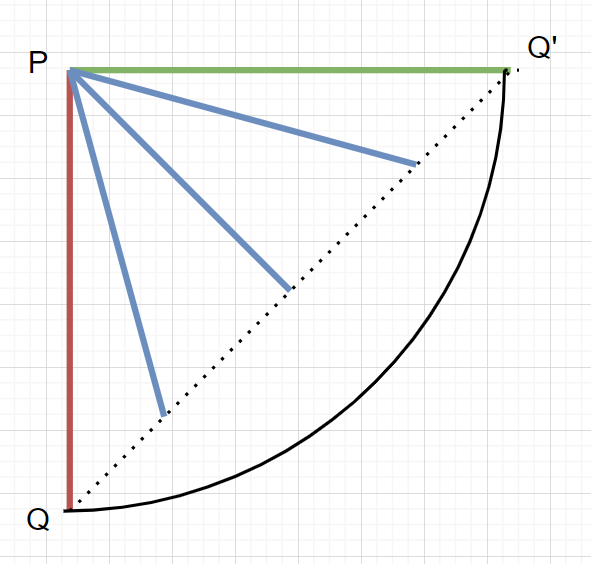
\includegraphics[width=0.8\textwidth]{linearinterpolation.drawio.png}
	\caption{Lineare Interpolation zwischen Ziellinie $\overline{PQ}$ und Quelllinie $\overline{PQ'}$}
	\label{fig:linearinterpolation}
\end{figure}
Durch diese Art der Interpolation entsteht jedoch bei
Rotationen ein Fehler, wie man in \ref{fig:linearinterpolation} sehen kann: Die linear
interpolierten Linien nehmen faelschlicherweise
an Laenge ab. In unseren praktischen Tests hat sich
dieses Problem als nicht gravierend herausgestellt. Durch die Linienpaare
laesst sich ein Pixel $\textbf{X}$ im Zielbild einem Pixel $\textbf{X'}$ zuordnen
(\ref{fig:xtoxprime}),
da durch das Paar eine Transformation festgelegt werden kann \cite{beierneely}.
Fuer unsere Implementierung nutzen wir den von Beier und Neely
mitgelieferten Pseudocode.

\begin{figure}[htb]
	\centering
	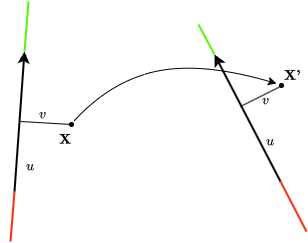
\includegraphics[width=0.8\textwidth]{xtoxprime.drawio.png}
	\caption{Transformation des Pixels $\textbf{X}$ nach $\textbf{X'}$}
	\label{fig:xtoxprime}
\end{figure}

\clearpage

\begin{minipage}{\textwidth}
\begin{lstlisting}[language=C++, caption=Beier-Neely in C++, label=bncode, xleftmargin=0.5cm]
for (uint32_t y = 0; y < destImage.m_Height; y++) {
	for (uint32_t x = 0; x < destImage.m_Width; x++) {
		glm::vec2 X = glm::vec2(x, y);
		glm::vec2 DSUM = glm::vec2(0.0, 0.0);
		float weightsum = 0;     
		for (uint32_t i = 0; i < destLines.size(); i++) {
			
			Line& destLine = destLines[i];
			Line& srcLine = sourceLines[i];
			Line interpolatedLine = InterpolateLinesLinear(destLine, srcLine, pct);
			
			glm::vec2 P = destLine.a.pos;
			glm::vec2 Q = destLine.b.pos;
			glm::vec2 srcP = interpolatedLine.a.pos;
			glm::vec2 srcQ = interpolatedLine.b.pos;
			glm::vec2 PX = X - P;
			glm::vec2 PQ = Q - P;
			float PQlength = glm::length(PQ);
			float u = glm::dot(PX, PQ) / (PQlength * PQlength);
			float v = glm::dot(PX, Perpendicular(PQ)) / PQlength;
			glm::vec2 srcPQ = srcQ - srcP;
			glm::vec2 srcX = srcP + u * srcPQ + (v * Perpendicular(srcPQ) / glm::length(srcPQ));
			glm::vec2 D = srcX - X;
			float dist = Distance(u, v, P, Q, X);
			float weight = glm::pow(glm::pow(PQlength, p) / (a + dist), b);
			DSUM += D * weight;
			weightsum += weight;        
		}                
		glm::vec2 srcX = X + DSUM / weightsum;
		if ((uint32_t)srcX.x > destImage.m_Width - 1) srcX.x = float(destImage.m_Width - 1);
		if ((uint32_t)srcX.y > destImage.m_Height - 1) srcX.y = float(destImage.m_Height - 1);
		if ((uint32_t)srcX.x < 0) srcX.x = 0.0f;
		if ((uint32_t)srcX.y < 0) srcX.y = 0.0f;                
		
		glm::ivec3 sourcePixel = sourceImage((uint32_t)srcX.x, (uint32_t)srcX.y);                
		
		unsigned char* newPixel = image.m_Data + (image.m_Channels * (y * image.m_Width + x));
		newPixel[0] = sourcePixel.r;
		newPixel[1] = sourcePixel.g;
		newPixel[2] = sourcePixel.b;
		
	} // ! pixel row
} // ! pixel col    
\end{lstlisting}
\end{minipage}



